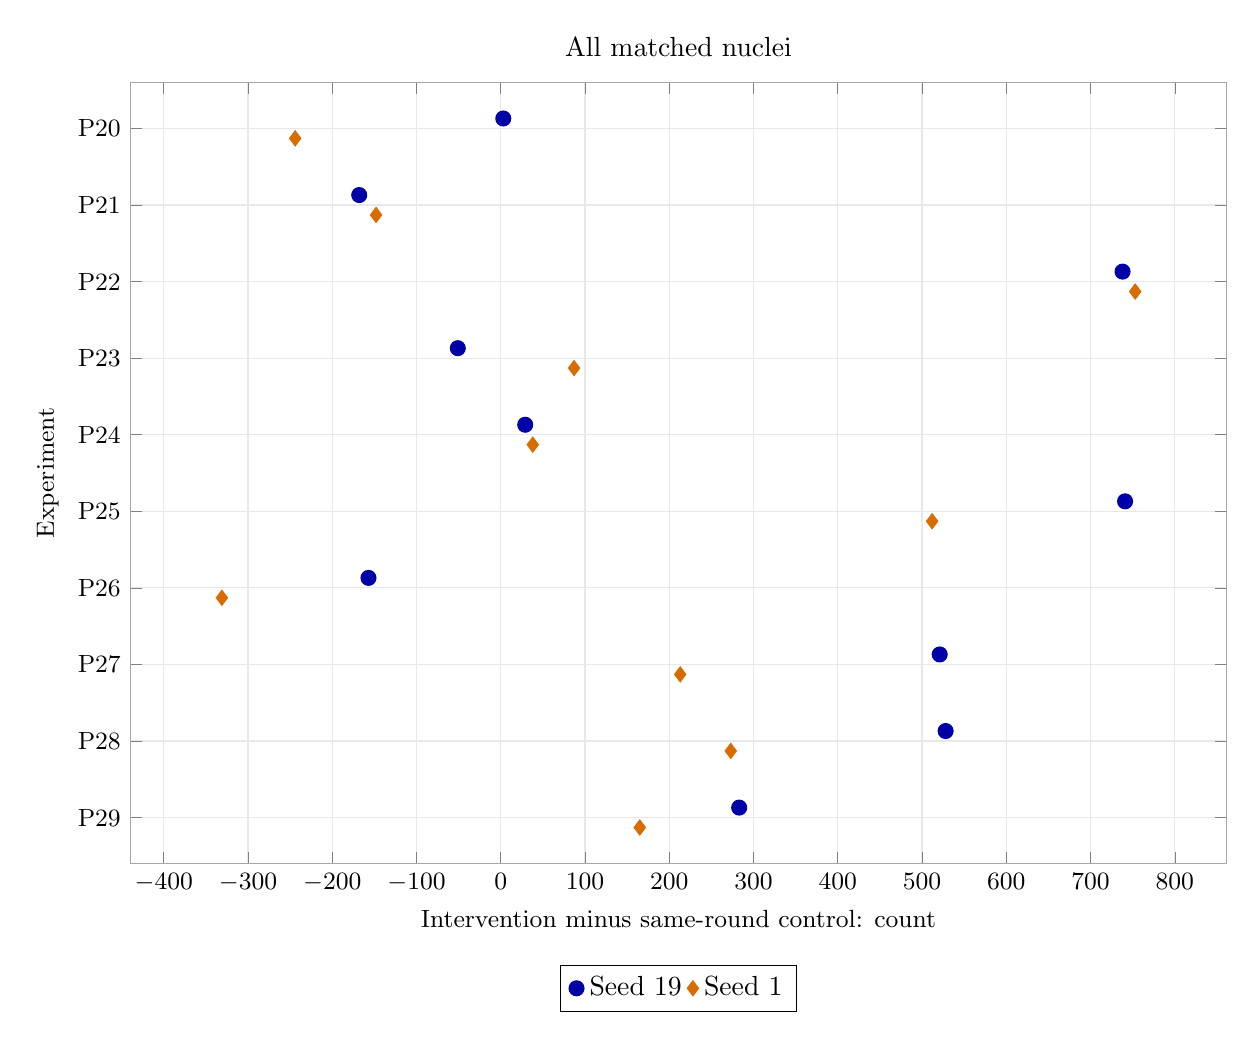
\begin{tikzpicture}
\begin{axis}[width=15.5cm,height=11.5cm,xlabel={Intervention minus same-round control: count},ylabel={Experiment},title={All matched nuclei},ytick={0,1,2,3,4,5,6,7,8,9},yticklabels={P20,P21,P22,P23,P24,P25,P26,P27,P28,P29},ymin=-.6,ymax=9.6,y dir=reverse,grid=major,grid style={gray!18},legend style={at={(.5,-.13)},anchor=north,legend columns=2},axis line style={gray!70},tick label style={font=\small},label style={font=\small},title style={font=\normalsize}]
\addplot[only marks,mark=*,mark size=2.7pt,color=blue!65!black] coordinates {(3,-0.13) (-168,0.87) (738,1.87) (-51,2.87) (29,3.87) (741,4.87) (-157,5.87) (521,6.87) (528,7.87) (283,8.87)};
\addlegendentry{Seed 19}
\addplot[only marks,mark=diamond*,mark size=2.7pt,color=orange!85!black] coordinates {(-244,0.13) (-148,1.13) (753,2.13) (87,3.13) (38,4.13) (512,5.13) (-331,6.13) (213,7.13) (273,8.13) (165,9.13)};
\addlegendentry{Seed 1}
\end{axis}
\end{tikzpicture}
